\documentclass[12pt]{article}

% packages

%\usepackage{times} % alt: cmbright
\usepackage[top=1in, bottom=1in, left=1in, right=1in]{geometry}
\usepackage{natbib}
\usepackage{amsmath}
\usepackage{amssymb}
\usepackage{latexsym}
\usepackage{sectsty}
\usepackage{amsfonts}
\usepackage{epsfig}
\usepackage{url}
\usepackage{microtype}
\usepackage{fixmath}
\usepackage{hyperref}
\usepackage{amsthm}
\usepackage{subfigure}
\usepackage{float}
\usepackage{hyperref}

\newtheorem{lem}{Lemma}
\newtheorem{defn}{Assumption}
\newtheorem{propty}{Property}
\newtheorem{thm}{Theorem}

% references

\newcommand{\mysec}[1]{Section~\ref{sec:#1}}
\newcommand{\myapp}[1]{Appendix~\ref{app:#1}}
\newcommand{\myeq}[1]{Equation~\ref{eq:#1}}
\newcommand{\myeqp}[1]{Eq.~\ref{eq:#1}}
\newcommand{\mychap}[1]{Chapter~\ref{chap:#1}}
\newcommand{\myfig}[1]{Figure~\ref{fig:#1}}

% math conveniences

\newcommand{\g}{\,\vert\,}
\newcommand{\E}{\textrm{E}}
\newcommand{\vct}[1]{\textbf{#1}}
\newcommand{\realline}{\mathbb{R}}
\newcommand{\indpt}{\protect\mathpalette{\protect\independenT}{\perp}}
\def\independenT#1#2{\mathrel{\rlap{$#1#2$}\mkern2mu{#1#2}}}
\newcommand{\h}[1]{\textrm{H}\left( #1 \right)}
\newcommand{\half}{\frac{1}{2}}
\newcommand{\new}{\textrm{new}}

\newcommand{\mult}{\textrm{Mult}}
\newcommand{\dir}{\textrm{Dir}}
\newcommand{\discrete}{\textrm{Discrete}}
\newcommand{\Bern}{\textrm{Bern}}
\newcommand{\DP}{\textrm{DP}}
\newcommand{\GP}{\textrm{GP}}
\newcommand{\Bet}{\textrm{Beta}}

% paragraph spacing

\setlength{\parindent}{0pt}
\setlength{\parskip}{2ex plus 0.5ex minus 0.2ex}

\allsectionsfont{\sffamily\mdseries}
\paragraphfont{\sffamily\bfseries}

\usepackage{algorithm}
\usepackage{algorithmic}
\renewcommand{\algorithmicrequire}{\textbf{Input:}}
\renewcommand{\algorithmicensure}{\textbf{Output:}}


\begin{document}

\title{\textsf{Approximating Multi-Objective Optimization using Particle Swarm}}
%\author{\textsf{Daqing Yi}}
\date{\textsf{Brigham Young University}}

\maketitle

\section{Multi-Objective Optimization}

Multi-objective optimization is a class of problems with solutions that can be evaluated along two or more incomparable or conflicting objectives.

Without loss of generality, we focus only on minimization objective in this paper. 
Because any minimum objective can be converted into a maximum objective by adding a negative operator, and vice verse. 

\begin{mydef}[\textbf{Multi-Objective Optimization}]
\label{def:multi_opt}
Find the vector $ \vec{x}^{*} \in S $ which will satisfy the $ m $ inequality constraints
\begin{equation}
\label{eq:mo_ineq_constraint}
g_{i}(\vec{x}) \geq 0, i = 1, 2, \cdots , m, 
\end{equation}
the $ p $ equality constraints
\begin{equation}
\label{eq:mo_eq_constraint}
h_{i}(\vec{x}) = 0, i = 1, 2, \cdots , p, 
\end{equation}
and will optimize the vector function
\begin{equation}
\label{eq:mo_obj}
\min_{ S } \vec{f}(\vec{x}) = \min_{ S } \left[ f_{1}(\vec{x}), f_{2}(\vec{x}) \cdots f_{k}(\vec{x}) \right]^{T},
\end{equation}
where $ \vec{x} $ is the vector of decision variables.
\end{mydef}

Here we would like to emphasize that there exists two spaces in a multi-objective optimization problem, which are
\emph{solution space} $ S \subset \mathbb{R}^{n}  $ and \emph{evaluation space} $ Z \subset \mathbb{R}^{k} $.
$ \vec{f}() $ maps a position $ x \in S $ to a position $ z \in Z $.

Due to the incomparability and conflict between objectives, there is usually no solution that satisfies all the objectives.
We import \emph{dominance} to describe a relationship between any two solutions.

\begin{mydef}[\textbf{Dominance}]
\label{def:dominance}
$ \vec{x} \in S $ dominates $ \vec{x'} \in S $, if 
\begin{equation}
\label{eq:def_dominance}
\forall i \in \{ 1, 2, \cdots k \}, f_{i}(\vec{x}) \leq f_{i}(\vec{x'}).
\end{equation}
We write it as $ \vec{x} \preceq \vec{x'} $.

$ \vec{x}  $ is non-dominant, if 
\begin{equation}
\label{eq:def_nondominant}
\nexists \vec{x'} \in S \land \vec{x'} \neq \vec{x}, \vec{x'} \preceq \vec{x}.
\end{equation}
\end{mydef}

A set of all the non-dominant solutions is called a \emph{Pareto set}.
\begin{mydef}[\textbf{Pareto set}]
\label{def:pareto_opt_set}
For a given multi-objective optimization problem $ \vec{f}() $, the \emph{Pareto optimal set} $ P^{*}_{S} \subset S $ is defined as
\begin{equation}
\label{eq:pa_opt_set}
P^{*}_{S} := \{ \vec{x} \in S \mid \nexists \vec{x}' \in S, \vec{x'} \preceq  \vec{x} \}.
\end{equation}

\end{mydef}

\emph{Pareto set} defines \emph{Pareto optimal} for the multi-objective optimization problems.
In the evaluation space $ Z $, we have a \emph{Pareto front} mapped from \emph{Pareto set} by $ \vec{f}() $.

\begin{mydef}[\textbf{Pareto Front}]
\label{def:pareto_front}
For a given multi-objective optimization problem $ \vec{f}() $ and Pareto optimal set $ P^{*}_{S} \subset S $, the \emph{Pareto front} $ P^{*}_{Z} \subset Z $ is defined as
\begin{equation}
\label{eq:pa_front}
P^{*}_{Z} := \{ \vec{z} = \vec{f}(\vec{x}) \mid \vec{x} \in P^{*}_{S} \}.
\end{equation}
\end{mydef}

\begin{figure} 
  \centering 
  \subfigure[Solution space]{ 
    \label{fig:sol_space} %% label for first subfigure 
    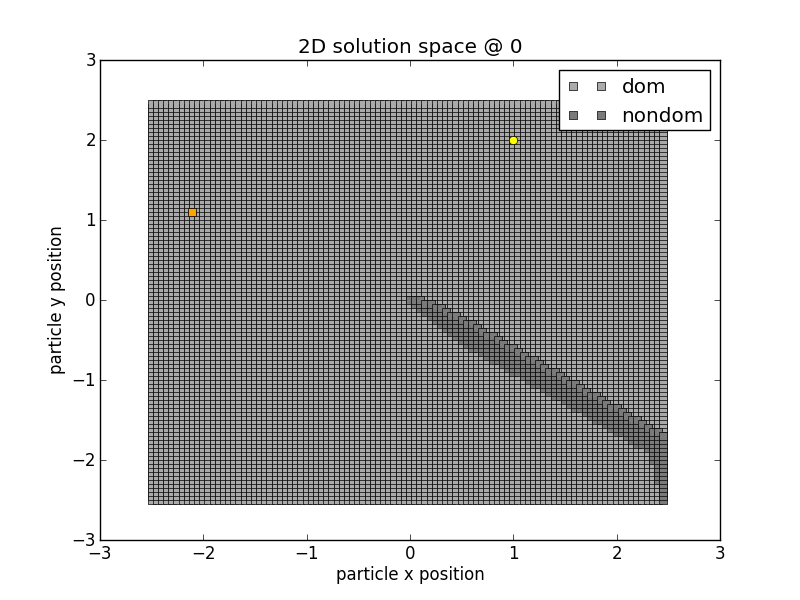
\includegraphics[width=0.45\textwidth]{./images/solution_space.png}} 
  %\hspace{1in} 
  \subfigure[Evaluation space]{ 
    \label{fig:eval_space} %% label for second subfigure 
    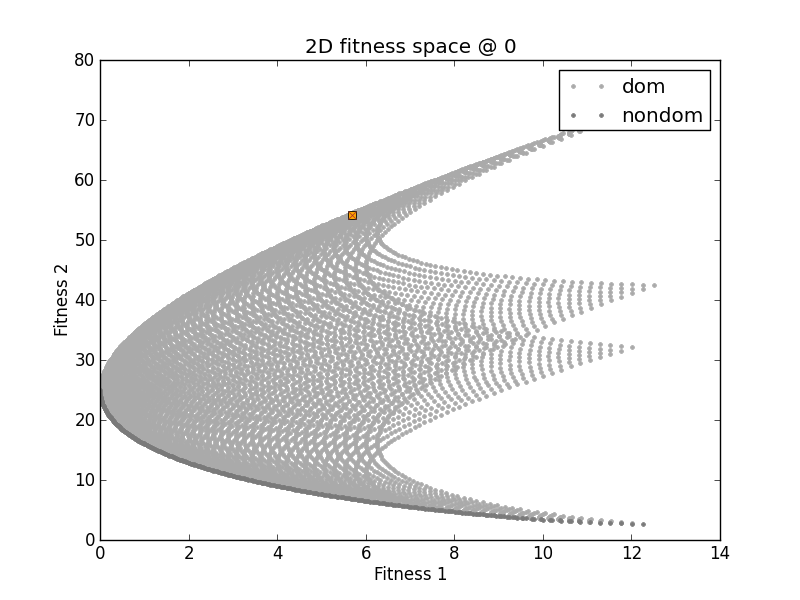
\includegraphics[width=0.45\textwidth]{./images/evaluation_space.png}}      
  \caption{Mapping between solution space and evaluation space.}
  \label{fig:space_mapping} %% label for entire figure 
\end{figure}

Due to how \emph{Pareto optimal} is defined, there is no straightforward way to solve like that in a conventional single-objective optimization problem.
Evolutionary algorithms are popular approaches to the multi-objective optimization problems. 

In this paper, we are interested with how to use \emph{Particle swarm optimization} to solve the multi-objective optimization problems.

\section{Particle Swarm Optimization}

\begin{mydef}[\textbf{Particle Swarm Optimization}]
\label{def:pso}

Let $ X $ be a set of particles.  
A \emph{particle} is a data structure that maintains current position $ \vec{x}_{i} $ and current velocity  $ \vec{v}_{i} $.
Denote $ \vec{x}^{P}_{i} $ for \emph{personal best}, which is the most fit position remembered of a particle. 
Denote $ \vec{x}^{G}_{i} $ for \emph{global best}, which is most fit $ \vec{x}^{P}_{i} $ among all particles. 
The algorithm runs as below:
\begin{enumerate}
\item Scattering particles $ \vec{x}_{i}(0) $ in decision space stochastically
\item Each particle update its location over time \\
\begin{equation}
\label{eq:up_vel}
\begin{aligned}
\vec{v}_{i}(t) & = \chi [ \vec{v}_{i}(t-1) + \phi^{P} \vec{u}^{P}_{i}(t-1) \otimes (\vec{x}^{P}_{i}(t-1) - \vec{x}_{i}(t-1)) \\
& + \phi^{G} \vec{u}^{G}_{i}(t-1) \otimes (\vec{x}^{G}_{i}(t-1) - \vec{x}_{i}(t-1)) ],
\end{aligned}
\end{equation}
\begin{equation}
\label{eq:up_pos}
\vec{x}_{i}(t) = \vec{x}_{i}(t-1) + \vec{v}_{i}(t),
\end{equation}
in which each element of $ \vec{u}^{P}_{i}(t-1) $ and $ \vec{u}^{G}_{i}(t-1) $ is independently sampled from uniform distribution $ [0, 1] $.
\end{enumerate}
\end{mydef}

In a multi-objective optimization problem, the particles are searching for a set instead of a position in the position space.
We extend the concept of ``global best'' and ``personal best'' from positions to sets of positions.
It means that each particle maintains a local estimation of the personal best set and the swarm maintains a global estimation of the global best set.
Like \cite{clerc2006stagnation} defined ``stagnation'' in a single objective problem, we define the stagnation in the multi-objective problem.
\begin{mydef}[\textbf{Stagnation of PSO in the Multi-Objective Optimization Problem}]
\label{def:mo_stagnation}
In a multi-objective optimization problem, we define that a particle is in \emph{stagnation stage} when the ``global best'' set and the ``personal best'' set are not changed.
\end{mydef}

We will analyze the behavior of a particle in stagnation in the next section.

\section{Stagnation Analysis}

\subsection{What happens when a particle is in stagnation}

THIS IS a mean square convergence.


If it converges, where it converges to.

\section{How to get better estimation}




\bibliographystyle{apalike}
\bibliography{reference}

\end{document}
